\begin{figure}[h]
\centering
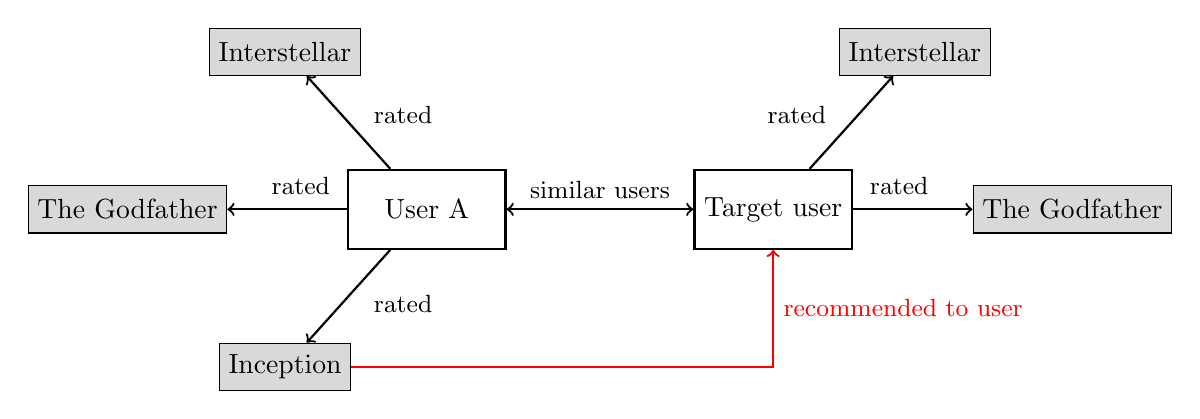
\begin{tikzpicture}[
    node distance=2cm,
    film/.style={circle, draw, minimum size=0.8cm, thick},
    user/.style={rectangle, draw, minimum width=2cm, minimum height=1cm, thick},
    movie/.style={rectangle, draw, minimum width=1.5cm, minimum height=0.6cm, fill=gray!30},
    arrow/.style={->, thick},
    redarrow/.style={->, thick, red},
    doublearrow/.style={<->, thick},
    label/.style={font=\small}
]
% Define positions
\coordinate (center) at (0,0);
% Users
\node[user] (userA) at (-2.2,0) {User A};
\node[user] (target) at (2.2,0) {Target user};
% Movies for User A (left side)
\node[movie] (int1) at (-4,2) {Interstellar};
\node[movie] (god1) at (-6,0) {The Godfather};
\node[movie] (inc1) at (-4,-2) {Inception};
% Movies for Target user (right side)
\node[movie] (int2) at (4,2) {Interstellar};
\node[movie] (god2) at (6,-0) {The Godfather};

% Arrows from movies to users
\draw[arrow] (userA) -- (int1);
\node[label] at (-2.5, 1.2) {rated};

\draw[arrow] (userA) -- (god1);
\node[label] at (-3.8, 0.3) {rated};

\draw[arrow] (userA) -- (inc1);
\node[label] at (-2.5, -1.2) {rated};

\draw[arrow] (target) -- (int2);
\node[label] at (2.5, 1.2) {rated};

\draw[arrow] (target) -- (god2);
\node[label] at (3.8, 0.3) {rated};

% Similar user connection
\draw[doublearrow] (userA) -- (target) node[midway, above, label] {similar users};
% Recommendation arrow
\draw[redarrow] (inc1) -- (2.2, -2) -- (target) node[midway, right, label] {recommended to user};
\end{tikzpicture}
\caption{User-based collaborative filtering. Similar users have similar rating histories.}
\label{fig:collaborative_filtering}
\end{figure}